% Jacobs Landscape Poster Version 1.1 (14/06/14)
\documentclass[final]{beamer}
\usepackage[scale=1]{beamerposter} % Use the beamerposter package for laying out the poster
\usetheme{confposter} % Use the confposter theme supplied with this template
\setbeamercolor{block title}{fg=ngreen,bg=white} % Colors of the block titles
\setbeamercolor{block body}{fg=black,bg=white} % Colors of the body of blocks
\setbeamercolor{block alerted title}{fg=white,bg=dblue!70} % Colors of the highlighted block titles
\setbeamercolor{block alerted body}{fg=black,bg=dblue!10} % Colors of the body of highlighted blocks

\newlength{\sepwid}
\newlength{\onecolwid}
\newlength{\twocolwid}
\newlength{\threecolwid}
\setlength{\paperwidth}{1189mm} % A0 width: 46.8in
\setlength{\paperheight}{846mm} % A0 height: 33.1in
\setlength{\sepwid}{0.01\paperwidth} % Separation width (white space) between columns
\setlength{\onecolwid}{0.22\paperwidth} % Width of one column
\setlength{\twocolwid}{0.46\paperwidth} % Width of two columns
\setlength{\threecolwid}{0.70\paperwidth} % Width of three columns
\setlength{\topmargin}{-0.5in} % Reduce the top margin size

\usepackage{graphicx}  % Required for including images
\usepackage{booktabs} % Top and bottom rules for tables
\usepackage{pstricks,pst-plot,pst-text,pst-tree,pst-eps,pst-fill,pst-node,pst-math}
\usepackage{algorithm,algorithmic}
\renewcommand{\algorithmicrequire}{\textbf{Input:}}
\renewcommand{\algorithmicensure}{\textbf{Output:}}

\title{Latent Dirichlet Allocation \medskip} % Poster title
\author{J\'er\^ome DOCK\`ES {\small{(\texttt{jerome@dockes.org})}}, Pascal LU  {\small{(\texttt{pascal.lu@centraliens.net})}} } % Author(s)
\institute{\'Ecole Normale Sup\'erieure de Cachan $-$ \today} % Institution

\begin{document}

\addtobeamertemplate{block end}{}{\vspace*{2ex}} % White space under blocks
\addtobeamertemplate{block alerted end}{}{\vspace*{2ex}} % White space under highlighted (alert) blocks

\setlength{\belowcaptionskip}{2ex} % White space under figures
\setlength\belowdisplayshortskip{2ex} % White space under equations

\begin{frame}[t] 
\begin{columns}[t]

%----------------------------------------------------------------------------------------
%	COLUMN 1
%----------------------------------------------------------------------------------------

\begin{column}{\sepwid}\end{column} % Empty spacer column

\begin{column}{\onecolwid}

\begin{alertblock}{Objectives}
We consider the problem of modeling text corpora. The goal is to find short descriptions of the members of a collection. Our work is mainly based on:
\nocite{*}
\small{\bibliographystyle{unsrt}\bibliography{sample}}
\end{alertblock}


\begin{block}{Notations}
\begin{itemize}
  \item $\mathcal{D} = \{d_{1},d_{2}, \ldots, d_{M}\}$ is a corpus.
  \item $\mathcal{V}$ is the vocabulary of size $V$.
  \item $k$ is the number of topics.
\end{itemize}

For a document $d \in \mathcal{D}$,
\begin{itemize}  
  \item $d = (w_1^{(d)}, \ldots, w_{N_d}^{(d)})$ represents the document $d$. $N_d$ is the number of words in the document $d$.
  \item $w^{(d)}$ is a matrix whose element $w_{ni}^{(d)} = 1$ if the word $n$ in the document is the word $i$ in the vocabulary. Size of $w^{(d)}$ = $N_d \times V$.
  %$w^{(d)}$ (\texttt{word$\_$incidences}) is a dictionary containing for each word (indexed by its position in the vocabulary) the number of times it appears in the document. Size of $w^{(d)}$ = $N_d \times 2$.
 \item $\theta^{(d)}$ is an array of size $k$, representing a probability density.
 \item $z^{(d)}$ is the set of topics : $z_{ni}^{(d)} =  1$ if the word $n$ was generated by the topic $i$. Size of $z^{(d)}$ $= N_d \times k$.
\end{itemize}
\end{block}

\begin{block}{Presentation of the model}
Latent Dirichlet allocation (LDA) is a generative probabilistic model of a corpus. 
\begin{itemize}
  \item Documents = random mixtures over latent topics,
  \item Topic = a distribution over words. 
\end{itemize} 

\medskip

\begin{algorithmic}[1]
\ENSURE corpus $\mathcal{D}$
\FOR{each document $d \in \mathcal{D}$}
\STATE Choose the length $\ell$ of $d$ $\sim \textnormal{Poisson}(\xi)$
\STATE Choose $\theta^{(d)} \sim \textnormal{Dir}(\alpha)$

\FOR{each of the $\ell$ words $w$}
\STATE Choose a topic $t \sim \textnormal{Multinomial}(\theta^{(d)})$
\STATE Choose a word $w$ from $p(w | t, \beta)$, a multinomial probability conditioned on $t$.
\ENDFOR
\ENDFOR
\end{algorithmic}

We have:
\begin{align*}
p(d|\alpha, \beta) 
& = \int p(\theta^{(d)}|\alpha) \left( \prod_{n=1}^{N_{d}} p(w_n^{(d)}|\theta^{(d)}, \beta)\right) \text{d}\theta  \\
& = \int p(\theta^{(d)}|\alpha) \left( \prod_{n=1}^{N_{d}} \sum_{z_n^{(d)}} p(z_n^{(d)}|\theta^{(d)}) p(w_n^{(d)}|z_n^{(d)}, \beta)\right) \text{d}\theta
\end{align*}

\end{block}

\end{column}


%----------------------------------------------------------------------------------------
% COLUMN 2
%----------------------------------------------------------------------------------------

\begin{column}{\sepwid}\end{column} % Empty spacer column
\begin{column}{\onecolwid}
\begin{block}{Generative model}
The goal is to determine:
\begin{itemize}
\item $\alpha$ is an estimate of the parameter of the Dirichlet distribution which generates the parameter for the (multinomial) probability distribution over topics in the document. Size of $\alpha = k$.

\emph{Exchangeable Dirichlet distribution} assumption: 
\[\forall i \in \{1, \ldots, k\}, \quad \alpha_i = \alpha\]
\item $\beta$ is a matrix of size $k \times V$ which gives the estimated probability that a given topic will generate a certain word: $\beta_{ij}= p(w^j = 1 | z^i = 1)$.
\end{itemize}

\begin{figure}[ht!]
\begin{center}
\psset{xunit=3cm,yunit=3cm,algebraic=true,dimen=middle,dotstyle=o,dotsize=5pt 0,linewidth=0.8pt,arrowsize=3pt 2,arrowinset=0.25}
\begin{pspicture*}(-0.5,-0.1)(8,3.4)
\rput(0,1){\pscirclebox[linecolor=black,fillstyle=solid,fillcolor=blue]{\textcolor{white}{$\alpha_j$}}}
\rput(2,1){\pscirclebox{$\theta^{(d)}_j$}}
\rput(4,1){\pscirclebox{$z^{(d)}_{nj}$}}
\rput(6,1){\pscirclebox[linecolor=black,fillstyle=solid,fillcolor=yellow]{$w_{nj}^{(d)}$}}
\rput(6,3){\pscirclebox[linecolor=black,fillstyle=solid,fillcolor=blue]{\textcolor{white}{$\beta_{jv}$}}}
\pspolygon(3.25,0.25)(7.2,0.25)(7.2,1.75)(3.25,1.75)
\pspolygon(1.25,0)(7.75,0)(7.75,2)(1.25,2)
\psline{->}(0.26,1)(1.6,1)
\psline{->}(2.41,1)(3.6,1)
\psline{->}(4.42,1)(5.6,1)
\psline{->}(6,2.7)(6,1.4)
\rput(6.75,0.5){$N_d$}
\rput(7.5,0.25){$M$}
\end{pspicture*}
\end{center}
\end{figure}
\end{block}

\begin{block}{Variational inference}

We need to compute the posterior distribution of the hidden variables given a document $d$:
\[ p(\theta^{(d)}, z^{(d)} | d, \alpha, \beta) = \frac{p(\theta^{(d)}, z^{(d)}, d | \alpha, \beta)}{p(d | \alpha, \beta)} \]
%$\Rightarrow$ Use Jensen's inequality to obtain a lower bound on the log likelihood.
For a document $d \in \mathcal{D}$:
 \begin{itemize}
  \item $\gamma^{(d)}$ is the variational parameter for the Dirichlet distribution. Size of $\gamma^{(d)}$ = $k$.
  \item $\phi^{(d)}$ is the variational parameter for the multinomial distribution. Size of $\phi^{(d)}$ = $N_d \times k$.
  
  $\phi_{ni}^{(d)}$ depends on the relation between the word in position $n$ of the document and the topic $i$ of the list of topics.
   \end{itemize}
\[ q(\theta^{(d)}, z^{(d)}|\gamma^{(d)}, \phi^{(d)}) = q(\theta^{(d)}|\gamma^{(d)}) \prod_{n=1}^{N_d} q(z_n^{(d)}|\phi_n^{(d)})\]
$\Rightarrow$ Estimate $\gamma^{(d)}, \phi_{n}^{(d)}$ instead of $\theta^{(d)}$ and $z_n^{(d)}$.
\[ (\gamma^{(d)}, \phi^{(d)}) = \mathop{\textnormal{argmin}}_{(\gamma, \phi)} \textnormal{D} \left( q(\theta^{(d)}, z^{(d)}|\gamma, \phi) \left\| p(\theta^{(d)}, z^{(d)} | d, \alpha, \beta) \right. \right) \]
\begin{figure}[ht!]
\begin{center}
\psset{xunit=2.75cm,yunit=2.75cm,algebraic=true,dimen=middle,dotstyle=o,dotsize=5pt 0,linewidth=0.8pt,arrowsize=3pt 2,arrowinset=0.25}
\begin{pspicture*}(-1,-0.1)(4,4)
\rput(0,3){\pscirclebox[linecolor=black,fillstyle=solid,fillcolor=green]{$\gamma^{(d)}_j$}}
\rput(0,1){\pscirclebox{$\theta^{(d)}_j$}}
\rput(2,3){\pscirclebox[linecolor=black,fillstyle=solid,fillcolor=green]{$\phi^{(d)}_{nj}$}}
\rput(2,1){\pscirclebox{$z^{(d)}_{nj}$}}
\pspolygon(1.25,0.25)(3.15,0.25)(3.15,3.75)(1.25,3.75)
\pspolygon(-0.9,0)(3.8,0)(3.8,4)(-0.9,4)
\psline{->}(0,2.6)(0,1.4)
\psline{->}(2,2.6)(2,1.4)
\rput(2.75,0.5){$N_d$}
\rput(3.5,0.25){$M$}
\end{pspicture*}
\end{center}
\end{figure}
\end{block}
\end{column}

%----------------------------------------------------------------------------------------
% COLUMN 3
%----------------------------------------------------------------------------------------

\begin{column}{\sepwid}\end{column} % Empty spacer column
\begin{column}{\onecolwid}

\begin{block}{Variational Inference Procedure \\ (E-step for a document $d$)}

\begin{algorithmic}[1]
\REQUIRE a document $d$ defined by its $w^{(d)}$, $\alpha, \beta$
\ENSURE $\gamma^{(d)}$, $\phi^{(d)}$

\STATE Initialize $\phi_{ni}^{(d)} = \frac{1}{k}$ for all $i$ and $n$.
\STATE Initialize $\gamma_i^{(d)} = \alpha + \frac{1}{k}\sum_{n=1}^{N_d} w_n^{(d)}$ for all $i$.
\WHILE{the expected log-likelihood $L(\gamma^{(d)}, \phi^{(d)}, \alpha, \beta)$ for the document $d$ has not converged}
\FOR{$n=1\ldots N_d$}
\FOR{$i=1\ldots k$}
\STATE $\phi_{ni}^{(d)} = \beta_{iw_n^{(d)}}\exp(\Psi(\gamma_i^{(d)}))$
\ENDFOR
\STATE Normalize $\phi_n^{(d)}$ to sum to $1$.
\ENDFOR
\STATE $\gamma^{(d)} = \alpha + \sum_{n=1}^{N_d} w_n^{(d)} \phi_n^{(d)}$
\STATE Update $L(\gamma^{(d)}, \phi^{(d)}, \alpha, \beta)$
\ENDWHILE
\end{algorithmic}
\end{block}


\begin{block}{EM-algorithm}

\begin{algorithmic}[1]
\REQUIRE corpus $\mathcal{D}$, number of topics $k$
\ENSURE $\alpha$, $\beta$

\FOR{each $d \in \mathcal{D}$}
\STATE Compute $w^{(d)}$.
\ENDFOR
\STATE Initialize $\alpha$ and $\beta$.

\WHILE{the expected log-likelihood $L(\alpha, \beta)$ has not converged}
\STATE Initialize $\Sigma_{\gamma} = 0$, $\beta_{\textnormal{new}} = 0$ and $L(\alpha, \beta) = 0$.
\FOR{each $d \in \mathcal{D}$}
\STATE $(\gamma^{(d)}, \phi^{(d)})$ = \textbf{variational-inference}$(w^{(d)}, \alpha, \beta)$
\STATE $\beta_{\textnormal{new}} \leftarrow \beta_{\textnormal{new}} + (\phi^{(d)})^{\top}w^{(d)}$
\STATE $\Sigma_{\gamma} \leftarrow \Sigma_{\gamma} + \sum_{i=1}^k \Psi (\gamma_i^{(d)}) - \Psi\left( \sum_{j=1}^k \gamma_j^{(d)}\right)$
\STATE $L(\alpha, \beta) \leftarrow L(\alpha, \beta) +L(\gamma^{(d)}, \phi^{(d)}, \alpha, \beta)$
\ENDFOR
\STATE Normalize $\beta_{\textnormal{new}}$ and set $\beta = \beta_{\textnormal{new}}$
\WHILE{$\alpha$ has not converged}
\STATE $\frac{\partial L}{\partial \alpha}(\alpha) = |\mathcal{D}| k \left[ \Psi\left( k \alpha \right) - \Psi(\alpha)\right] + \Sigma_{\gamma}$
\STATE $\frac{\partial^2 L}{\partial \alpha^2}(\alpha) = |\mathcal{D}|k [k\Psi'(k\alpha) - \Psi' \left( \alpha\right)]$
\STATE $\alpha \leftarrow \alpha - \frac{\frac{\partial L}{\partial \alpha}(\alpha)}{\frac{\partial^2 L}{\partial \alpha^2}(\alpha)}$
\ENDWHILE
\ENDWHILE
\end{algorithmic}
\end{block}

\begin{block}{Implementation issues}
\begin{itemize}
  \item \textbf{Document and vocabulary preprocessing}.
  \item $\alpha > 0$ and $\beta$ were initialized randomly.
  \item \textbf{Representation of $w^{(d)}$}: $N_d$ is the number of \textbf{distinct} words in the document $d$ and $w^{(d)}$ is a dictionary containing for each distinct word (indexed by its position in the vocabulary) the number of times it appears in the document. Size of $w^{(d)}$ = $N_d \times 2$.
 
%  \item Under the exchangeable Dirichlet distribution assumption, the computation of $\alpha$ becomes much simpler.

\end{itemize}
\end{block}
\end{column}

%----------------------------------------------------------------------------------------
% COLUMN 4
%----------------------------------------------------------------------------------------

\begin{column}{\sepwid}\end{column} % Empty spacer column
\begin{column}{\onecolwid}
\begin{block}{Results}
We tested our LDA on real data from the Reuters21578 database (\texttt{reut2-000.sgm}).

\begin{table}
\vspace{2ex}
\begin{footnotesize}
\begin{tabular}{ccccc}
\toprule
\textbf{Topic 1} & \textbf{Topic 2} & \textbf{Topic 3}  & \textbf{Topic 4} & \textbf{Topic 5}\\
\midrule
devices & prolonged & zestril & seasons & withdrawn \\
disk & council & annesthetic &  hotels & expiration  \\
megabyte & forum & hypertension & VMS & clearances \\
expandable & dissident & oth & Biltmore  & expire \\
megabytes & flying & statil & Marriott & Willemijn \\
equipped &  sparks & diabetic & rename & BV \\
monochrome &talks & complications & hotel & Rotterdam  \\
peripheral & outweighed & Barbara & 228 & licensed \\
color & accomplishments & definitive & DH  & NCR \\
\bottomrule
\end{tabular}
\end{footnotesize}
\caption{Results for 5 topics $(k=20)$}
\end{table}

\begin{figure}[ht!]
\begin{center}
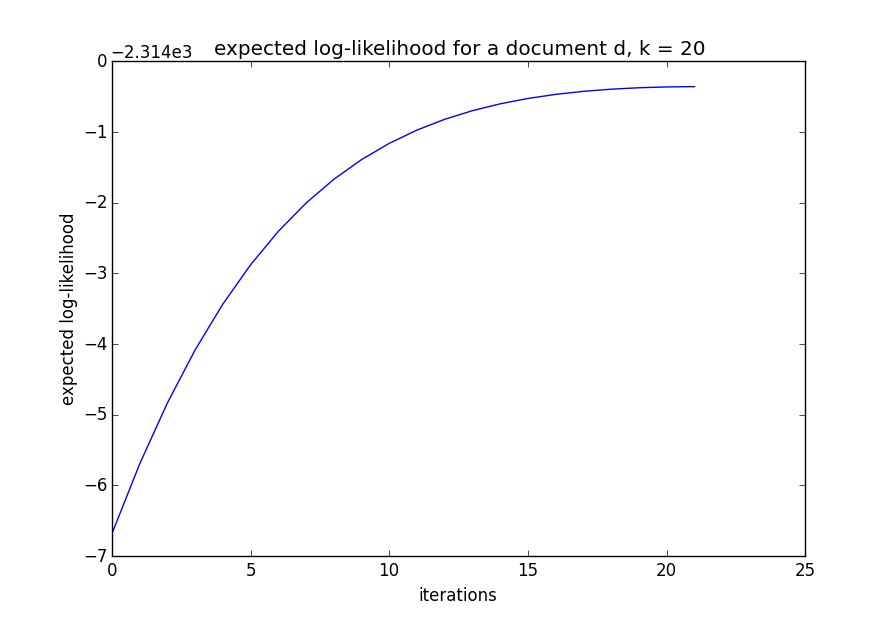
\includegraphics[width=0.7\linewidth]{../img/k=20/log_likelihood_document_k=20.png}
\caption{Expected log-likelihood for a document ($k=20$)}
\end{center}
\end{figure}

\begin{figure}[ht!]
\begin{center}
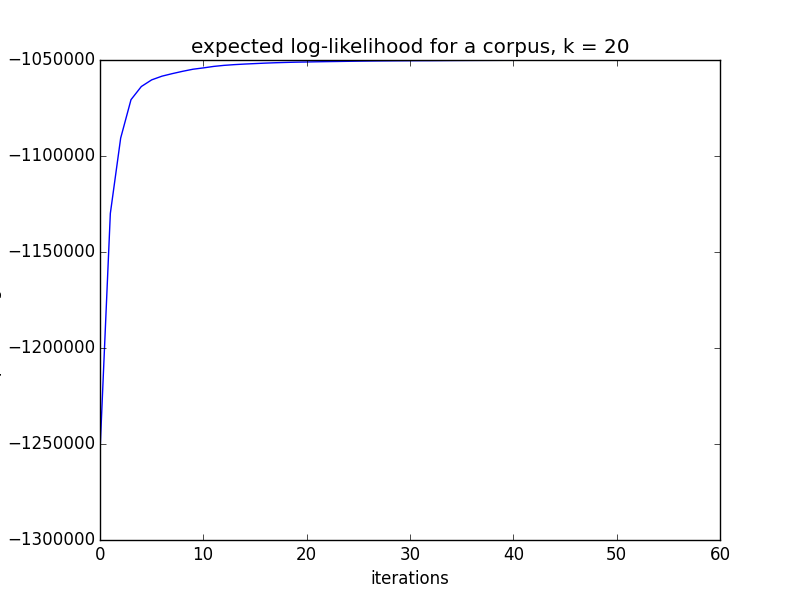
\includegraphics[width=0.7\linewidth]{../img/k=20/log_likelihood_corpus_k=20.png}
\caption{Expected log-likelihood for the corpus ($k=20$)}
\end{center}
\end{figure}
\end{block}

\begin{block}{Conclusion}
\begin{itemize}
  \item LDA = a way to apply graphical models to information retrieval = group words in the same categories. 
  \item Key idea = variational inference. 
  \item LDA is a non-convex optimization problem: estimates for $\alpha, \beta$ depend on their initialization.
  \item Other interesting applications: biology (DNA sequence), content-based image retrieval$\ldots$
\end{itemize}
\end{block}

%\begin{block}{References}
%\nocite{*}
%\small{\bibliographystyle{unsrt}
%\bibliography{sample}\vspace{0.75in}}
%\end{block}

\setbeamercolor{block alerted title}{fg=black,bg=norange}
\setbeamercolor{block alerted body}{fg=black,bg=white}
%\begin{alertblock}{Contact Information}
%\begin{itemize}
%  \item \texttt{jerome\{at\}dockes.org}
%  \item \texttt{pascal.lu\{at\}centraliens.net}
%\end{itemize}
%\end{alertblock}
\end{column}

\end{columns} % End of all the columns in the poster
\end{frame} % End of the enclosing frame

\end{document}
